\section{LruCache}\label{sec:lru}

\begin{figure}
\begin{center}
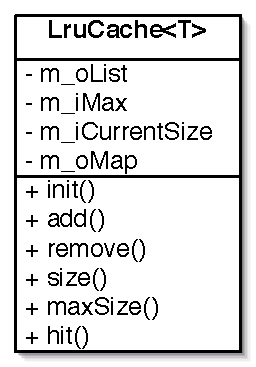
\includegraphics[width=0.4\textwidth]{figs/lru}
\end{center}
\caption{}
\label{fig:lru}
\end{figure}

This section describes the LruCache component, which is described by Figure~\ref{fig:lru}.  The LRU cache is a simple template class that
implements a Least Recently Used eviction policy for its entries.  It is configurable to have a maximum size and has simple accessors and an
init function.  It uses an STL map<> class to to store its data and an custom list class that supports random access.

\subsection{Methods}

{\bf Public Methods}
\begin{itemize}
\item init(): This method initializes all of the internal state.  This method takes an optional parameter that specifies the maximum size
that the cache may grow.
\item add(): This method takes a template type <T> and adds it to the internal structures.
\item remove(): This method removes an object from the cache.
\item size(): This method returns the current size of the cache.
\item maxSize(): This method returns the upper limit on how large the cache may grow.
\item hit(): This method is used to lookup an entry in the cache and move it to the most recently used if it exists.
\end{itemize}

\subsection{Member Variables}
\begin{itemize}
\item m\_oList
\item m\_iMax
\item m\_iCurrentSize
\item m\_oMap
\end{itemize}
